% THIS IS SIGPROC-SP.TEX - VERSION 3.1
% WORKS WITH V3.2SP OF ACM_PROC_ARTICLE-SP.CLS
% APRIL 2009
%
% It is an example file showing how to use the 'acm_proc_article-sp.cls' V3.2SP
% LaTeX2e document class file for Conference Proceedings submissions.
% ----------------------------------------------------------------------------------------------------------------
% This .tex file (and associated .cls V3.2SP) *DOES NOT* produce:
%       1) The Permission Statement
%       2) The Conference (location) Info information
%       3) The Copyright Line with ACM data
%       4) Page numbering
% ---------------------------------------------------------------------------------------------------------------
% It is an example which *does* use the .bib file (from which the .bbl file
% is produced).
% REMEMBER HOWEVER: After having produced the .bbl file,
% and prior to final submission,
% you need to 'insert' your .bbl file into your source .tex file so as to provide
% ONE 'self-contained' source file.
%
% Questions regarding SIGS should be sent to
% Adrienne Griscti ---> griscti@acm.org
%
% Questions/suggestions regarding the guidelines, .tex and .cls files, etc. to
% Gerald Murray ---> murray@hq.acm.org
%
% For tracking purposes - this is V3.1SP - APRIL 2009

\documentclass{acm_proc_article-sp}
% these seem necessary to get 8.5x11 (letter) page size working in pdflatex
\setlength{\pdfpagewidth}{8.5in}
\setlength{\pdfpageheight}{11in}
\usepackage[export]{adjustbox}
\usepackage[bookmarks, pdfborderstyle={/S/U/W 0}]{hyperref}
\usepackage{minted}
\usepackage{caption}
\usepackage{tikz}
%%% This file is generated by Makefile.
%%% Do not edit this file!
%%%
\def\githash{0eb3347*}


\usemintedstyle{friendly}
\newminted{json}{linenos=false, stepnumber=1, frame=lines, framesep=1em}

\newenvironment{tightitemize}{
    \vspace{-10pt}
    \begin{itemize}
        \setlength{\parskip}{-1pt}}{
    \end{itemize}
    \vspace{-10pt}}

\newenvironment{tightenumerate}{
    \vspace{-10pt}
    \begin{enumerate}
        \setlength{\parskip}{-1pt}}{
    \end{enumerate}
    \vspace{-10pt}}

% command from http://www.acm.org/sigs/publications/sigfaq
\def\sharedaffiliation{
\end{tabular}
\begin{tabular}{c}}

\begin{document}

\title{Hypermedia APIs for Sensor Data}
\subtitle{A pragmatic approach to the Web of Things}
\toappear{Submitted to 11th International Conference on Mobile and Ubiquitous
          Systems: Computing, Networking and Services (Mobiquitous 2014)\\
          December 2-5, 2014\\
          London, Great Britain\\
          Build \githash}

% You need the command \numberofauthors to handle the 'placement
% and alignment' of the authors beneath the title.
%
% For aesthetic reasons, we recommend 'three authors at a time'
% i.e. three 'name/affiliation blocks' be placed beneath the title.
%
% NOTE: You are NOT restricted in how many 'rows' of
% "name/affiliations" may appear. We just ask that you restrict
% the number of 'columns' to three.
%
% Because of the available 'opening page real-estate'
% we ask you to refrain from putting more than six authors
% (two rows with three columns) beneath the article title.
% More than six makes the first-page appear very cluttered indeed.
%
% Use the \alignauthor commands to handle the names
% and affiliations for an 'aesthetic maximum' of six authors.
% Add names, affiliations, addresses for
% the seventh etc. author(s) as the argument for the
% \additionalauthors command.
% These 'additional authors' will be output/set for you
% without further effort on your part as the last section in
% the body of your article BEFORE References or any Appendices.

\numberofauthors{2}

%  You can go ahead and credit any number of authors here,
%  e.g. one 'row of three' or two rows (consisting of one row of three
%  and a second row of one, two or three).
%
%  The command \alignauthor (no curly braces needed) should
%  precede each author name, affiliation/snail-mail address and
%  e-mail address. Additionally, tag each line of
%  affiliation/address with \affaddr, and tag the
%  e-mail address with \email.

\author{
% 1st author
\alignauthor Spencer Russell\\
    \email{sfr@media.mit.edu}
% 2nd author
\alignauthor Joseph A. Paradiso\\
    \email{joep@media.mit.edu}
\sharedaffiliation
    \\
    \affaddr{Responsive Environments Group}  \\
    \affaddr{MIT Media Lab}   \\
    \affaddr{Massachusetts Institute of Technology} \\
    \affaddr{Cambridge, MA, USA}
}

%\author{
%% 1st author
%\alignauthor Author One\\
%    \email{author1@example.com}
%% 2nd author
%\alignauthor Author Two\\
%    \email{author2@example.com}
%\sharedaffiliation
%    \\
%    \affaddr{Research Group}  \\
%    \affaddr{Research Institution} \\
%    \affaddr{Research Location}
%}

\date{14 July 2014}

\maketitle

\begin{abstract}
As our world becomes more instrumented, sensors are appearing in our homes,
cars, and on our bodies~\cite{dublonsciam}. These sensors are connected to a
diverse set of systems and protocols driven by cost, power, bandwidth, and
more. Despite this heterogeneous infrastructure, we need to be able to build
applications that use that data, and the most value comes from integrating
these disparate sources together. Infrastructure for the Internet of Things is
becoming more commonplace, but we need an application layer to enable
interoperability and create a \emph{Web} of Things. Here we introduce a
pragmatic approach to the Web of Things, integrating HTTP request/response
interactions with realtime streaming using HTML5 WebSockets.  We will discuss
how our approach enables client/server interactions that are both evolvable by
the server and discoverable by the client. Rather than attempt to define yet
another competing standard, we incorporate a collection of complementary
standards already in use. We will also describe our implementation of these
concepts in ChainAPI, a sensor data server in use by a variety of projects
within our research group.  We will describe one of several end-to-end
applications as a successful case study.
\end{abstract}

% % A category with the (minimum) three required fields
% \category{H.4}{Information Systems Applications}{Miscellaneous}
% %A category including the fourth, optional field follows...
% \category{D.2.8}{Software Engineering}{Metrics}[complexity measures, performance measures]
%
% \terms{Theory}
%
\keywords{Semantic Web, RESTful Web Services, Sensors, Internet of Things, Hypermedia, Linked Data} % NOT required for Proceedings

\section{Introduction}

It is becoming apparent that in addition to a transport layer that enables the
Internet of Things, it is important to develop an application layer to provide
wide-spread interoperability and a consistent interface to Internet-connected
devices. While there are many efforts to develop new standards and
protocols such as Alljoyn and MQTT, other projects~\cite{guinard2010} seek to
use existing application-level web standards such as HTTP to provide an
interface that is more familiar to developers, and also that can take advantage
of tooling and infrastructure already in place for the World Wide Web.
Reflecting the relationships to existing web standards and also the way in
which the World Wide Web is built on top of the Internet, these efforts are
often dubbed the Web of Things.

In previous work~\cite{doppellab}\cite{gestures} we have built frameworks to collect
and process sensor data from a variety of sources, as well as applications to
visualize and experience those data. Through these prototypes we identified
several common use cases and access patterns, as well as shared functionality
that would be better served by a common infrastructure.

We posit that the main impediments to adoption of IoT standards are social
rather then technological. Often solutions require developers to take on too much
simultaneous complexity to get started. Many of the systems coming from a Semantic
Web history have sophisticated data models to ensure compatibility with existing
upper ontologies~\cite{w3contology}\cite{broring2011}\cite{eid2007}, but
application developers are often unwilling to adopt this accompanying
complexity. Providing simple, familiar interfaces to sensor data lowers
the barriers to entry to building sophisticated applications without deep
knowledge of the underlying sensor architecture, enabling smarter, more
efficient IoT systems~\cite{aldrich2013}.

To address these issues we have developed ChainAPI, a sensor data server that
interoperates easily with existing infrastructure, and also allows developers
to take advantage of semantic relations and formal ontologies as they become
useful, rather than forcing the developer to confront them all at once. We are
working with developers outside our research group to get insight and feedback
into the barriers to adoption and also which features are necessary to cover
real-world use cases.

\section{Hypermedia Web Services}

One of the most influential works in Hypermedia Web Services is Roy Fielding's
PhD dissertation ``Architectural Styles and the Design of Network-based
Software Architectures''~\cite{fielding}. Fielding codified much of the design
that had gone into the World Wide Web into an architectural framework he called
Representational State Transfer, or REST. He lists the main requirements that
drove the design of the World Wide Web:

\begin{tightitemize}
    \item Low barrier to entry
    \item Extensibility
    \item Distributed hypermedia
    \item Internet-scale
\end{tightitemize}

The Internet of Things certainly must be extensible and Internet-Scale. This
work focuses on exploring the benefits of lowering barriers to entry and
hypermedia. While reducing complexity and providing easy entry points for new
developers are obviously good goals in isolation, there is often a trade-off
between design complexity and the expressive power and generality of a system.
However, the World Wide Web gives a compelling model of a system that has
proved itself to be both accessible (driving wide and rapid adoption) and
extensible. Guinard, Trifa, and Wilde give a good introduction to the
application of RESTful design to the Web of Things~\cite{guinard2010}.

\section{Using Existing Standards}

Wherever possible we have relied on existing standards and protocols rather
than reinventing our own. For instance, to support hypermedia in our responses
we are using the Hypertext Application Language~\cite{json-hal-draft}, which
provides a standardized data model for hyperlinks. HAL can be rendered in JSON
with a mediatype of \texttt{application/hal+json} or XML
(\texttt{application/hal+xml}). In this case we have chosen to focus on the JSON
variant. We use the IANA-standardized link relations \texttt{edit-form} and
\texttt{create-form} to indicate link relations that can be used for editing
and creating resources, and JSON-Schema~\cite{json-schema-draft} for
representing the expected format.

\begin{listing}
\begin{jsoncode}
  {
    "updated": "2014-04-01T02:34:21.676564+00:00",
    "dataType": "float",
    "metric": "sht_temperature",
    "value": 25.59,
    "_links": {
      "ch:dataHistory": {
        "href": "/sensordata/?sensor_id=274",
        "title": "Data"
      },
      "curies": [
        {
          "href": "/rels/{rel}",
          "name": "ch",
          "templated": true
        }
      ],
      "self": {
        "href": "/sensors/274"
      },
      "ch:device": {
        "href": "/devices/33",
        "title": "Office Thermostat"
      },
      "ch:websocketStream": {
        "href": "ws://example.com/ws/sensor-274",
        "title": "Websocket Stream"
      },
      "editForm": {
        "deprecation": "/rels/deprecation/editForm",
        "href": "/sensors/274/edit",
        "title": "Edit Sensor"
      },
      "edit-form": {
        "href": "/sensors/274/edit",
        "title": "Edit Sensor"
      }
    },
    "unit": "celsius"
  }
\end{jsoncode}
\caption{hal+json representation of a sensor}
\label{sensorjson}
\end{listing}

\section{Link Relations}

Hyperlinks provide a mechanism for the server to present
affordances~\cite{gibson} to the client. These affordances could represent
actions that the client has available to them, or simply related resources. For
example, a temperature sensor resource might have a link relation to a
thermostat setpoint, representing a target value. Non-numeric sensor data such
as RFID can link to the detected item or person. Linked resources could also be
virtual sensors such as an anomaly detection algorithm that uses raw sensor
data as input. Actions such as editing the current resource or sending a
command can also be represented as links, and the presence or absence of those
links is a way for the server to communicate to the client what they are
allowed to do. Listing \ref{sensorjson} has a typical resource representation.
In hal+json links are contained in a reserved \texttt{\_links} property of your
json payload. The \texttt{\_links} property is a dictionary, keyed on link
relation names (commonly referred to as ``rels'').

The rel itself actually serve as a link(URI) to the human-readable
documentation that describes what that relationship actually means. This rel
URI should also be used by clients as a unique, persistent identifier. This
gives flexibility to server implementers as they can add new relation types, or
even new versions of existing relation types, to existing resources without
breaking older clients. As long as the new rels have unique URIs, old clients
will simply ignore them. It also provides a mechanism for creating a shared
vocabulary of relation types by referencing rels from a shared repository.

Using URIs as relation names has the benefit of providing a stable and unique
identifier for relation names, but using a full URI as a json dictionary key is
cumbersome and duplicates lots of data in a typically payload. To alleviate this
issue hal+json supports Compact URIs or CURIEs, which are similar in
functionality to an XML namespace. In the context of hal+json CURIEs are simply
a URI template that can be used for each rel that references it. For example,
in Listing \ref{sensorjson} the \texttt{ch} CURIE has a templated URI of
\texttt{/rels/\{rel\}}, so the rel \texttt{ch:device} becomes
\texttt{/rels/device}. This substitution is known as CURIE Expansion.

Actions such as posting new sensor data or adding a new sensor require the
client to send data to the server. The client can send data to the server via
\texttt{POST} requests with data encoded in the body of the request with JSON.
The server can provide the client with the expected format of the data using
JSON-Schema~\cite{json-schema-draft}. A \texttt{GET} request to the given
relation will generate a response with the expected schema, and a \texttt{POST}
will edit or create the resource, depending on the relation.

You can also see in Listing \ref{sensorjson} that there is both an
\texttt{editForm} and \texttt{edit-form} relation. Notice that the
\texttt{editForm} link has a \texttt{deprecation} property that is a URI.  This
is how relations can be gracefully deprecated or changed. In this case we
renamed \texttt{editForm} to \texttt{edit-form} to match the IANA-registered
relation name. Older clients with the old relation name will continue to
function normally, and most HAL libraries are configured to log a warning if a
deprecated link relation is used. The deprecation URI can be viewed for
information about the deprecation. Developers creating new clients can clearly
see which relations are deprecated and avoid using them. HAL allows server
developers to decide on a deprecation lifetime policy appropriate for their
application.

To save on communication overhead, HAL also supports embedded resources as a
pre-caching strategy~\cite{json-hal-draft}. If there are related resources that
are likely to be requested, they can be included in an \texttt{\_embedded}
property that is similar in structure to the \texttt{\_links} property, except
with full HAL resources included instead of links. When a client application
accesses a related resource, most HAL client libraries are configured to first
check for the \texttt{\_embedded} before requesting the resource over the
network.

\section{Layered Architecture}

Work is under way by multiple groups to adapt the TCP/IP Stack to be more
suitable for low-power, resource-constrained devices~\cite{iotsurvey}. Though
this is a reasonable proposition and would provide a suitable transport
protocol for communication, it leaves open many questions that are important
for secure and reliable communication over the open Internet. Even if the
devices themselves speak IP (whether using WiFi, 6LoWPAN, etc.) there will
still likely be a role for a bridge or gateway node that can handle encryption,
authentication, discovery mechanisms, and other application logic necessary to
communicate and interoperate with the larger Internet.

One of the benefits of the layered gateway approach is that we can take
advantage of existing HTTP Caching and Proxy infrastructure. It is a common
pattern in modern web development to have application web server processes
handling application logic, and to place a front-end HTTP server such as Nginx
or Apache as a reverse proxy or gateway.  In this configuration, the proxy is
responsible for handling SSL encryption, defending against DDOS attacks, and in
general provides a front line of defense to the open Internet. The application
server processes (e.g.  Node.js or Gunicorn) thus operate in a safer
environment and focus on handling application logic.

The presence or absence of a gateway has been used in Web of Things literature
to divide direct from indirect integration~\cite{wotsurvey}. In direct
integration, the devices themselves are capable of serving requests directly
from clients. In indirect integration there is a gateway or bridge that serves
the requests, and translates them to a protocol that the (presumably
lower-powered) nodes can understand. An unexplored middle ground is for end
devices to function as simple HTTP servers that are proxied behind more complex
ones. For example, a gateway could handle SSL and authentication, but then
forward requests to the simpler devices for handling application logic. This
layered architecture is one of the six constraints that define the REST
architecture~\cite{fielding}, and allows the simpler devices to sit behind a
protected firewall in a safe zone. By building our simpler servers on HTTP we
can use industry-standard and field-tested front-end proxy servers instead of
special purpose IoT gateways.

The standard HTTP methods (\texttt{GET}, \texttt{POST}, etc.) have well-defined
semantics~\cite{httpmethods}. For instance, a \texttt{GET} request should have
no side effects in the server, and a \texttt{PUT} request should be idempotent
(making the request more than once has the same effect as making it once i.e.
the request can be safely repeated). Using these standard methods and adhering
to the defined semantics allows intermediate servers to behave more
intelligently and route traffic more efficiently. One notable example is the
caching proxy. There exist many widely-used proxies such as
Varnish\footnote{https://www.varnish-cache.org/},
Nginx\footnote{http://nginx.org/}, and
Squid\footnote{http://www.squid-cache.org/} that can take advantage of the HTTP
method along with standardized cache lifetime HTTP headers to intercept the
request and serve a cached response from a previous request, reducing the load
on the application server, which might otherwise have needed to access a
database or do other expensive calculations to re-build the response. In the
case of sensors the caching proxy could be a power-saving measure, as the proxy
could handle client requests without communicating with the sensor.

\section{Bringing Poll and Push\\ Together}

In ChainAPI we integrated request/response interactions with realtime push
updates. While many interactions map well to a Hypermedia HTTP API in which
clients make a request and the server sends a response, it is very common in
sensor data systems to want new sensor data as soon as it is available.
Standard HTTP is not well-suited to this task, the server cannot initiate
communication with the client. While many workarounds such as long-polling are
in common use, HTML5 WebSockets were introduced to eliminate the need for such
workarounds.

Clients begin interacting with ChainAPI via the HTTP API, submitting HTTP
requests for resources and receiving responses with representations of those
resources in hal+json. In a response, the server may provide a realtime feed
for related data simply by providing a \texttt{ch:websocketStream} link
relation. For example, in Listing \ref{sensorjson} the server is telling the
client that there is a WebSocket stream for this sensor available at
\texttt{ws://example.com/ws/sensor-274}. As new data from the sensor is
available it will be streamed to all subscribed clients. Because there is a
natural hierarchy in our data (many devices in a Site, usually several sensors
in each Device), when clients subscribe to a resource they get updates for all
resources below them in the hierarchy.

Another option with some traction is MQTT~\cite{collina2012}, which is
optimized for resource-constrained devices and includes useful features such as
variable Quality of Service levels and the ability to register a message to be
sent on disconnect, known as the ``last will and testament.'' For our
applications these have not been necessary and the simplicity of integrating
WebSockets with standard HTTP has proved beneficial. If in the future we decide
to support additional streaming protocols such as MQTT we can simply add new
link relations to allow clients to connect via those protocols, analogous to
the \texttt{ch:websocketStream} relation we currently use for the WebSocket
stream. Clients that support the new stream type will be able to take advantage
of it when the rel is available, and older clients will simply ignore the new
capability.

\section{Enabling Search}
\label{search}

In the early days of the World Wide Web, sites were primarily accessed directly
via their URIs, or via links from other known sites. In the earliest days in
fact, CERN had an alphabetized index of available web
content~\cite{websearchengines}. As the web grew beyond what could be
reasonably browsed and bookmarked, the problem of finding information on the
Web changed. It was no longer enough for the content to be on the web, it also
had to be discoverable in a sea of other pages. By 1994 search engines started
to appear to allow users to find the information they wanted. With search
engines came the advent of crawlers that would index the web and collect the
metadata into the engine's database.

As more sensors and sensor networks are added to the Web of Things, similar
issues will arise. Our approach can serve as a substrate on which a similar
ecosystem of crawlers can index the available data and metadata. Search engines
have also been one of the spaces where semantic markup is beginning to be
adopted and used,  as the engines use embedded semantic information in pages to
improve their results.

\section{Naming}

One of the central issues in the IoT is simply the issue of uniquely
identifying objects in the system~\cite{iotsurvey}. RESTful design practices
encourage HTTP URIs as globally unique identifiers. Providers can structure
their URIs arbitrarily, for instance to represent natural hierarchy in the
system. Link relations between objects not only represent identity, but also
where the linked object can be found, without needing to first consult any sort
of central registry. This architecture supports extremely loose coupling
between related resources and services.

Additionally, HTTP has built-in mechanisms to handle renaming, as servers can
respond with an HTTP Status 301 (Moved Permanently) to notify clients that the
object can now be found at a new URI.

\section{Supporting Relation Ontologies}

An ontology is a formal description of objects, classes, and concepts in a
domain, as well as the relations between them~\cite{gruber1993}. In the
Semantic Web context the entities in an ontology are typically defined as a set
of widely-available URIs so that unrelated actors and systems can reference
shared concepts~\cite{bernerslee2001semantic}. In fact, it's this ontological
common ground that enables the most powerful aspects of semantically-linked
data. Client agents can take data from disparate sources and leverage the
ontology to combine it meaningfully, for example combining temperature data
from multiple sources, or automatically combining sensor data from different
systems that it knows are nearby a particular latitude and longitude.

Implementing a fully Semantic Web-compatible system is not a priority of
ChainAPI, but we recognize the benefits of shared ontologies to support
cross-system compatibility. Hal+json and ChainAPI can use a shared vocabulary
of link relations to enable these types of use cases. In Listing
\ref{sensorjson}, notice the \texttt{ch:dataHistory} link relation, which
expands (via the CURIE) to the URI \texttt{/rels/dataHistory}. A client that
sees and understands this relation knows that it will link to a collection of
data from the history of this resource. A user-facing client might open the
link in a separate window that can graph the data. A M2M agent such as an
indexing crawler might choose to ignore the link because it is only concerned
with sensor metadata and not the actual measurements themselves. Perhaps it
will link back to the source for the raw data, while storing the metadata in a
more optimized index for the types of queries it will run.

In addition to acting as a universally-unique identifier, the rel name is also
a URI that can be dereferenced by the client to get more information on the
relation semantics. The human-readable documentation available at that URI is
useful during development, but machine-readable documentation can also be made
available, such as a JSON-Schema. This machine-readable information could be
used by a hypermedia client to display more information about the relation to
the user, or to decide whether or not to follow the relation in an M2M context.

Where possible we are using existing standard relation names. Some that apply
to the wider web are defined by the IANA, such as \texttt{next},
\texttt{previous}, \texttt{edit-form}, etc. There are currently several
available approaches to an ontology for sensor
data~\cite{w3contology}\cite{broring2011}\cite{eid2007} but they typically
focus on interoperating with more universal upper ontologies and are too
complex for use by general web developers. Other work on integrating various
ontologies with other existing sensor description standards such as SensorML
are promising~\cite{russomanno2005}, but finding the right balance between
simplicity and semantic expressivity remains an open research area.

A shared vocabulary of relation types is one part of the semantic picture, but
for a fully self-describing service it is also necessary for the client to
access information about the resource formats themselves. The IANA defines the
\texttt{profile} relation name that can be used to link individual resources to
a shared type that can be used as a context for interpreting its attributes.

\section{API Description}

To validate our design choices and experiment in a real-world environment, we
have implemented a server-side web service called ChainAPI. We have also
created several client applications to use the service in different ways.

ChainAPI is released under the MIT license, and source code is available on
GitHub\footnote{https://github.com/ssfrr/chain-api}.

\subsection{Resources}
\label{api_resources}

Following hypermedia design practice[cite], ChainAPI provides clients with a
number of resources and describes relations between them in the form of
hyperlinks. The resource types we currently provide are:

\begin{description}
    \item[Site] A collection of Devices typically located within the same
        geographic area or building.
    \item[Device] A physical device in an enclosure. This device could contain
        many sensors.
    \item[Sensor] A single metric that is measured, such as temperature or humidity.
    \item[SensorData] Raw data captured by the sensor.
\end{description}

Any resource can have a \texttt{geoLocation} property which contains its
latitude, longitude, and optionally elevation. Resources without a
\texttt{geoLocation} property inherit that of their parent.

\subsection{HTML Interface}

\begin{figure}
    \centering
    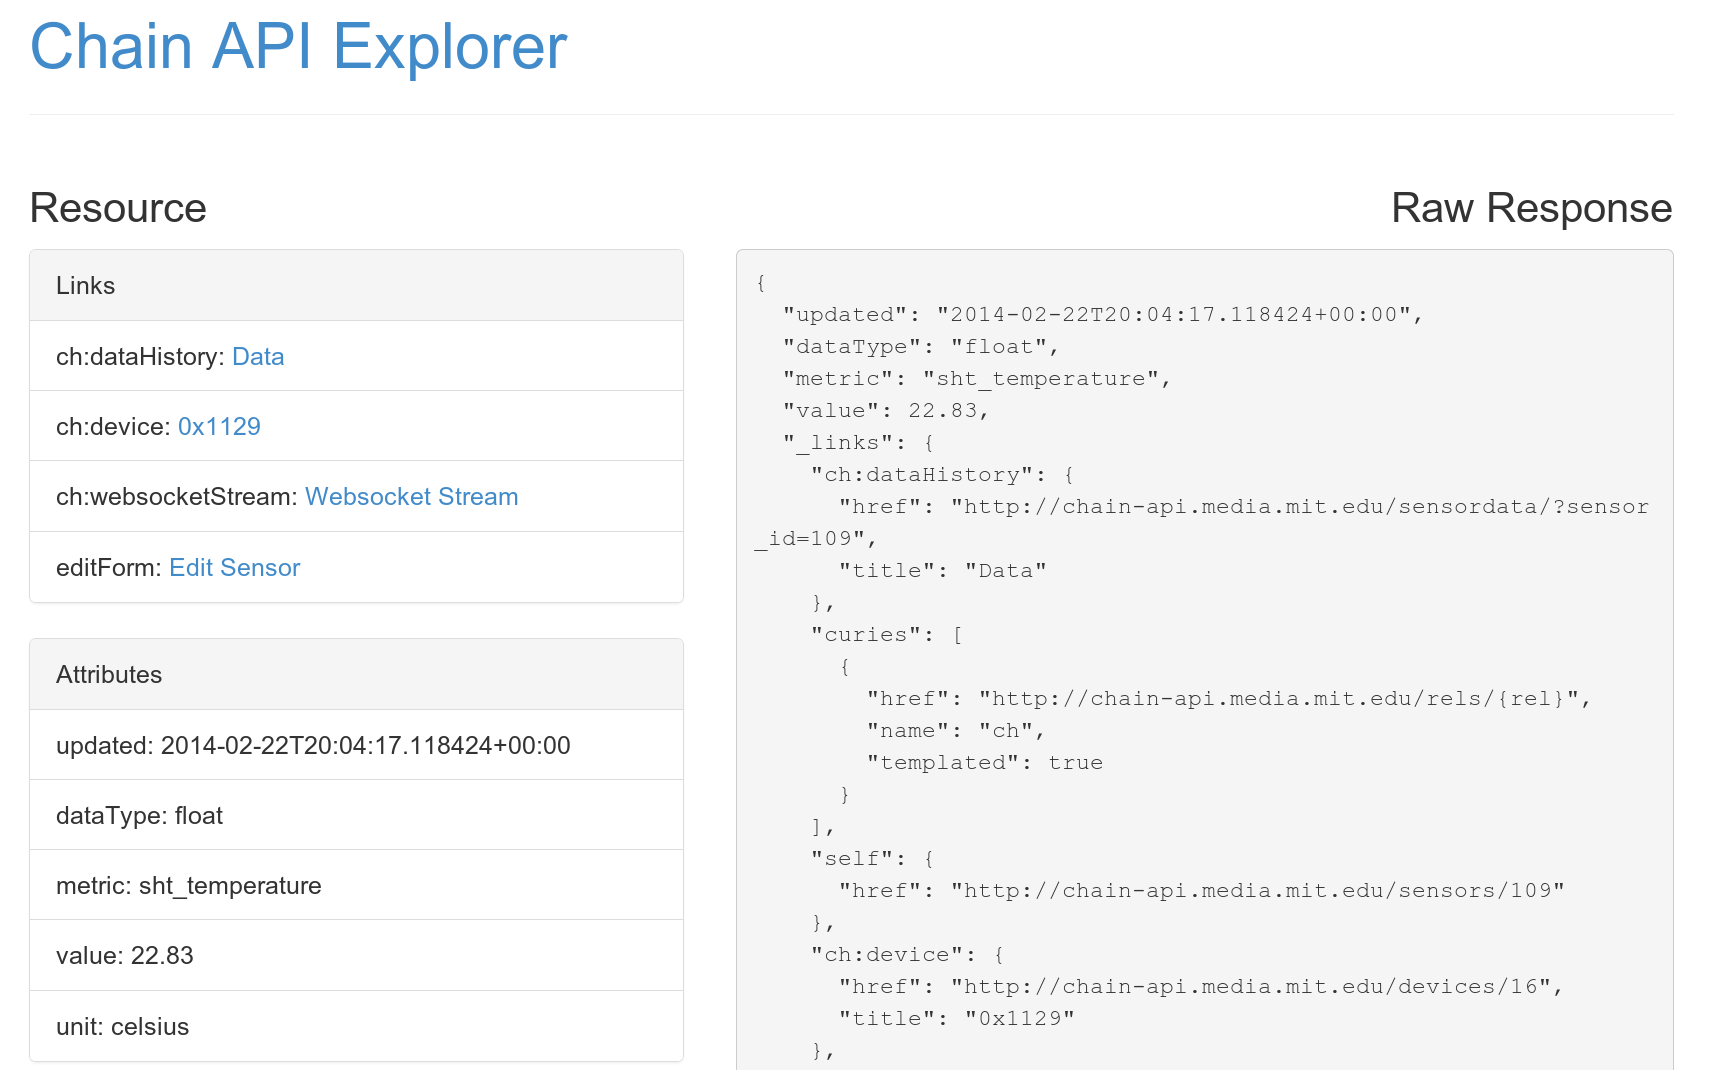
\includegraphics[width=8.45cm, frame]{chain_explorer2}
    \caption{Chain API Explorer}
    \label{chain_explorer}
\end{figure}

To assist developers building applications on top of ChainAPI, we have
developed a human-facing interface with HTML, CSS, and Javascript that can be
viewed through a standard web browser, as seen in Figure \ref{chain_explorer}.
Through this interface developers can familiarize themselves with the ChainAPI
interface before they start their client application, or to evaluate ChainAPI
for their application. For each request, we display the raw JSON of the
response on the right side. On the left we display a more user-friendly and
interactive rendering of the raw data.

Our HTML interface has the following capabilities

\begin{tightenumerate}
    \item Display resource attributes
    \item Display links as clickable HTML links
    \item Create and \texttt{POST} an HTML form from a JSON-Schema
    \item Plot time-series data on a graph
\end{tightenumerate}

Capabilities 1-3 are enough to enable a user to fully interact with the API
without any specialized code on the client side. Plotting time-series data is a
convenience to help visualize the data, but is not a core requirement of client
libraries. As new features and capabilities are added to the server, they
automatically become available in the client interface with no client-side code
changes.

\section{Implementation}

Our current implementation of the ChainAPI server is written in Python. We use
the Django\footnote{https://www.djangoproject.com/} web framework for the
request/response API and database interactions and a separate process built on
the Flask\footnote{http://flask.pocoo.org/} web framework for managing the
WebSocket connections. The two processes communicate with each other through a
ZMQ socket for event notification. We are currently using the
PostgreSQL\footnote{http://www.postgresql.org/} relational database. Nginx acts
as a reverse-proxy server to dispatch standard HTTP and also WebSocket
connections to the application servers.

It is currently only possible to create or modify resources through the HTTP
interface, but in the future clients will be able to use WebSockets to reduce
latency and overhead. When a client posts new data, for example a sensor
posting a new temperature measurement, the HTTP server handles persisting the
data in the database and also sends an event notification over ZMQ to the
WebSocket server, which in turn notifies any subscribed clients. The URI
provided to the client in the WebSocket links provides all the information the
WebSocket server needs to decide what data should be sent to the client. For
example, in the sensor resource in Listing \ref{sensorjson}, the WebSocket URI
is \texttt{ws://example.com/ws/sensor-274}, so when the client connects to the
WebSocket server, it will send any events tagged \texttt{sensor-274}.

While are certainly a long way from Internet-scale, we have a substantially
larger installation then most comparable research systems. As of August 7, 2014
there are 366 devices in the system, which include 1121 separate sensors. We
have collected over 100,000,000 sensor data measurements.

\section{Case Study:\\Tidmarsh Living Observatory}

The Tidmarsh Living Observatory project\footnote{http://tidmarshfarms.com/} is
a sensor deployment at a former cranberry bog in southern Massachusetts that is
currently undergoing a restoration to a natural wetland. There are currently 15
sensors nodes deployed, each sensing temperature, humidity, barometric
pressure, and ambient light. Each node is powered by 3 AA batteries, with an
expected battery life of 2 years, sampling every 20 seconds. Approximately 100
additional nodes will be installed in the coming months. Figure
\ref{tidmarsh_arch} shows an overview of the Tidmarsh architecture.

\begin{figure}
    \centering
    % load the library when editing in QTikZ, comment out for inclusion in the paper
%\usetikzlibrary{positioning}
\begin{tikzpicture}[
	sensornode/.style={
		shape=rectangle,
		draw,
		minimum size=10mm,
		rounded corners,
	},
	gateway/.style={
		shape=rectangle,
		draw,
		rounded corners,
		minimum width=25mm,
		minimum height=10mm,
	},
	server/.style={
		shape=rectangle,
		draw,
		rounded corners,
		minimum width=25mm,
		minimum height=10mm,
		text width=22mm,
		align=center,
	},
	client/.style={
		shape=circle,
		draw
	},
	>=stealth,
	->,
	thick,
	font=\footnotesize,
	node distance=7mm,
]
% draw the bounding rectangle
%\draw (0,0) rectangle (8.45, 10);

\node (n4) [sensornode] at (2.5,1) {Node};
\node (n5) [sensornode, right=of n4] {Node};
\node (n7) [sensornode, above=of n4] {Node};
\node (n6) [sensornode, left=of n7] {Node};
\node (n8) [sensornode, right=of n7] {Node};
\node (gateway) [gateway, above=of n7] {TCP/IP Gateway};
\node (zmq server) [server, above=of gateway] {Binary $\to$ JSON Translator};
\node (zmq json server) [server, above=of zmq server] {ZMQ $\to$ ChainAPI\\Bridge};

\node (client1)[client, right=of zmq json server] {Client};
\node (client2)[client, right=of client1] {Client};
\node (client3)[client, below=of client2] {Client};
\node (chain server) [server, above =of client1, yshift=10] {ChainAPI Server};

\draw[dashed] (n4) -- (n7);
\draw[dashed] (n5) -- node[right] {Atmel LWM (802.15.4)}(n8);
\draw[dashed] (n6) -- (gateway);
\draw[dashed] (n7) -- (gateway);
\draw[dashed] (n8) -- (gateway);

\draw (gateway) -- node[right] {ZMQ (binary)} (zmq server);
\draw (zmq server) -- node[right] {ZMQ (JSON)} (zmq json server);
\draw (zmq json server) -- node[left] {HTTP} (chain server);
\draw[<->] (client1) -- (chain server);
\draw[<->] (client2) -- node[right, text width=2cm, yshift=1.5mm] {HTTP, \\WebSockets} (chain server);
\draw[<->] (client3) -- (chain server);
\end{tikzpicture}

    \caption{Tidmarsh Architecture}
    \label{tidmarsh_arch}
\end{figure}

\subsection{Sensor Infrastructure}

One of the goals of ChainAPI is to accommodate a wide variety of heterogeneous
underlying sensor systems and provide easy integration. In the case of Tidmarsh
there was an existing sensor installation that exposed the sensor data via
ZMQ\footnote{http://zeromq.org/}.The sensors communicate with a base station
using Atmel's Lightweight Mesh protocol over 802.15.4. Nodes not within direct
communication range of the base station can route messages through
solar-powered router nodes, which are also collecting data. The base station
serves as the TCP/IP Gateway, which receives the RF messages and sends them
over WiFi to server via ZMQ. The message payloads are left in their binary
format and they are received by the Binary to JSON translator, which parses the
binary messages and generates JSON representations of the data. The Binary to
JSON translator acts as a ZMQ server, and the JSON messages are sent to any
connected clients.

\subsection{ChainAPI Representation}

To integrate the Tidmarsh sensor installation into ChainAPI, we wrote a small
bridge service that connects via ZMQ to the Tidmarsh server and receives JSON
messages on each sensor measurement. The only URI needed by the service
is the address of the Tidmarsh Site resource on the ChainAPI server, which is
passed as an argument on initialization. On initialization the bridge service
first requests a list of all Devices on the server. Recall from section
\ref{api_resources} that a Device is a collection of sensors in the same
enclosure, so in this case each Tidmarsh Node is a device. Within the Tidmarsh
system each node has a unique 2-byte identifier, which we use as the device's
name field within ChainAPI. From the device and sensor information that the
bridge receives from the server, it builds a hash that it can use to look up
the URI for a given sensor data as it arrives from the Tidmarsh server. It then
subscribes to the ZMQ feed from the Tidmarsh server. As new data come in, the
bridge simply looks up the appropriate URI to post the new data to. If data
arrives from a sensor or device that the bridge does not recognize, the bridge
creates the necessary resource before beginning to post data. This has the
benefit that as new sensors come online at Tidmarsh, their data immediately
begins flowing into ChainAPI.

\subsection{Client Behavior}

\begin{figure}
    \centering
    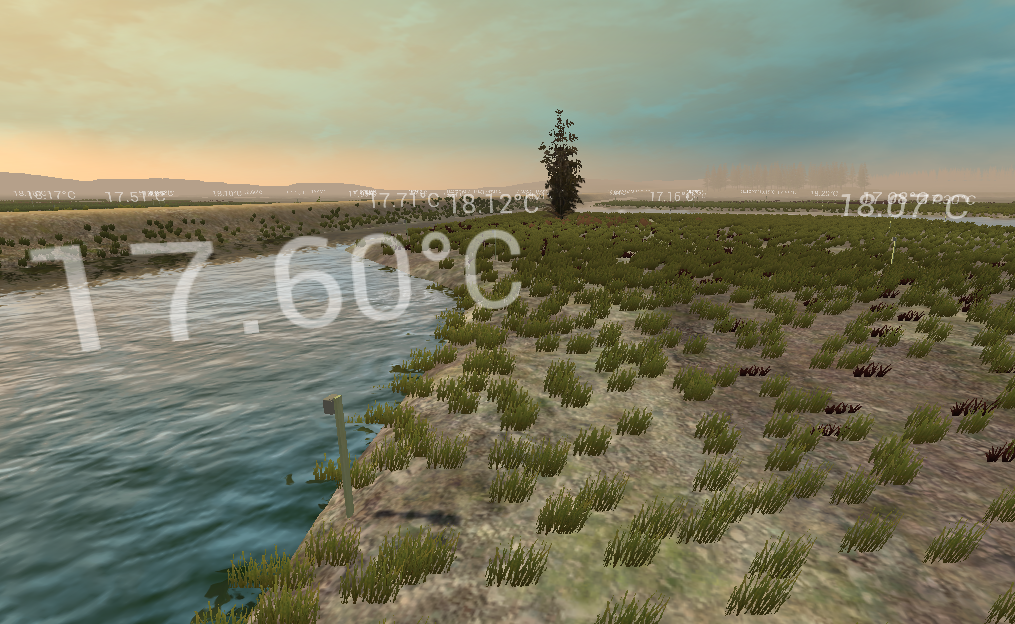
\includegraphics[width=8.45cm]{tidmarsh_screenshot}
    \caption{Tidmarsh Unity3D Client}
    \label{tidmarsh_screenshot}
\end{figure}

We developed an interactive 3D client built on the Unity3D game
engine\footnote{http://unity3d.com/} to explore and experience the data from
the sensor network. As with the Tidmarsh bridge, the client begins by
requesting a summary of the site, which includes all devices and sensors at
that site. Similar to the bridge, this client builds a hash to map incoming
data, but now in the opposite direction. New data that comes in from the
WebSocket subscription will have a link to the containing sensor, so the client
needs to quickly map that URI into an in-memory object representing the sensor.
As the client parses the summary of devices and sensors at the site, it builds
up such a map and instantiates the objects in the game world. As new data comes
in, the client looks up the game object in the hash and updates the sensor
values. In this client the incoming data is visualized and displayed spatially
on a realistic representation of the real-world topology (see
Figure~\ref{tidmarsh_screenshot}). The client also incorporates generative
music that is driven by the incoming sensor data. To maintain portability and
security, working within the Unity3D environment places substantial constraints
on library availability. Here the choice to use standard web technologies sped
up development time considerably. With no tooling or language support beyond
standard HTTP, WebSocket, and JSON parsing we were able to quickly interface
with the ChainAPI server and access the data in realtime.

\section{Future Work}

A general pattern has emerged in the clients we've built where they often begin
with one or more requests for the current state of the resources of interest,
after which they subscribe to push updates. The gap between the initial state
query and the push updates presents a potential for lost data. One solution
would be for the client to subscribe to the updates before requesting the
initial state, thus pushing responsibility for merging out-of-order data to the
client. Because this pattern is so common a better solution is desirable.
Because the initial state information and the WebSocket link for updates are
often in the same response, we should be able to include timestamp information
in the WebSocket link itself, which the WebSocket server can use on a new
client connection to send any messages that otherwise would have been lost.
Because the clients treat link URIs as opaque we can add this functionality to
the server at a later time without changes to the client.

The ontology that has arisen from our applications is underdeveloped and
ad-hoc. While we have discussed how a shared vocabulary could be implemented
within our system, more research is necessary to determine a widely-usable set
of relations, preferably based on existing ontologies and standards.

Much of this work is predicated on the assumption that we should strive to
simplify the client/server interfaces in Web of Things to drive adoption. To
validate this assumption we need to build in our qualitative experience with
formal user studies.

We have not yet explored the best security models to apply to this
architecture. Building on existing web technologies gives us access to a wealth
of proven security tools and paradigms, but we need to work on implementing
more fine-grained access control while maintaining the scalability advantages
such as caching.

There are many issues surrounding efficient handling of time-series data that
we have not yet addressed. Efficient querying at large time scales will require
working with the data at multiple resolutions. Downsampling the raw data brings
up many questions that require further research including effective ways to
handle missing data.

As discussed in Section \ref{search}, The web provides a successful model to
handle massive decentralized growth in the form of search engines. A collection
of hyperlinked sensor data forms a substrate for a more sophisticated ecosystem
of crawlers, aggregators, portals, etc. that can be extremely loosely-coupled
to the underlying data. It also enables these engines to index the data to
optimize for different use cases. Exploring this space is a rich avenue for
future research.

\section{Conclusion}
In this work we have introduced a number of design principles that can be used
together to build Web of Things applications that are extensible and scalable
while maintaining low barriers to entry and interfaces that are familiar to the
modern web developer. We have described ChainAPI, our implementation
demonstrating and validating that these ideas can support quick development
cycles for sensor network applications, and easily integrate with existing
infrastructure. We have achieved these goals using almost entirely existing
protocols and standards brought together in a unified architecture based on
REST and Hypermedia principles. This approach also supports data sharing and
interoperability through a shared vocabulary of link relations. With such a
proliferation of standards and protocols for the Internet of Things the
challenge becomes integrating the pieces into a coherent whole, and ChainAPI
is a concrete step in that direction.

%ACKNOWLEDGMENTS are optional
\section{Acknowledgments}
We would like to thank Cisco Systems, who provides partial funding for this
project.

% The following two commands are all you need in the
% initial runs of your .tex file to
% produce the bibliography for the citations in your paper.
\bibliographystyle{abbrv}
\bibliography{refs} % refs.bib is the name of the Bibliography in this case
%
% ACM needs 'a single self-contained file'! For final submission paste the contents
% of refs.bbl here.
%
\end{document}
